% !TEX TS-program = pdflatex
% !TeX program = pdflatex
% !TEX encoding = UTF-8
% !TeX spellcheck = en_US

\documentclass[11pt, a4paper]{article}
%\usepackage{fullpage}
\usepackage[left=1cm,right=1cm,top=1cm,bottom=2cm]{geometry}
\usepackage[fleqn]{amsmath}
\usepackage{amssymb}
%\usepackage{indentfirst}
\usepackage[T1]{fontenc}
\usepackage[utf8]{inputenc}
\usepackage[french,english]{babel}
\usepackage{txfonts} 
\usepackage[]{graphicx}
\usepackage{multirow}
\usepackage{hyperref}
\usepackage{parskip}
\usepackage{multicol}
\usepackage{wrapfig}

\usepackage{turnstile}%Induction symbole

\usepackage{tikz}
\usetikzlibrary{arrows, automata}
\usetikzlibrary{decorations.pathmorphing}

\renewcommand{\baselinestretch}{1}

\setlength{\parindent}{24pt}


\begin{document}

%\selectlanguage {french}
%\pagestyle{empty} 

\noindent
\begin{tabular}{ll}
\multirow{3}{*}{
\includegraphics[width=1.5cm]{../../../extra/logo/esi.nlp.pdf}} & \'Ecole national Supérieure d'Informatique\\
& 2\textsuperscript{nd} year second cycle (2CSSID)\\
& NLP: Natural Language Processing (2022-2023)
\end{tabular}\\[.25cm]
\noindent\rule{\textwidth}{2pt}\\[-0.5cm]
\begin{center}
{\LARGE \textbf{Lab04: Plagiarism detection}}
\begin{flushright}
	Abdelkrime Aries
\end{flushright}
\end{center}\vspace{-0.5cm}
\noindent\rule{\textwidth}{2pt}

We want to implement a simple plagiarism program using two sentence representations: TF and CBOW centroid. 

\section{Program description}

Our objective is to create a program which compares two text files sentence by sentence.
The comparison is based on cosine similarity between the sentences' encoding.
We want to use two sentence encoding methods: term frequency and CBOW centroid.
Our architecture is illustrated as a simple class diagram in figure \ref{fig:program}.
The bold red attributes and methods must be completed by the students. 

\begin{figure}[htp!]
	\centering
	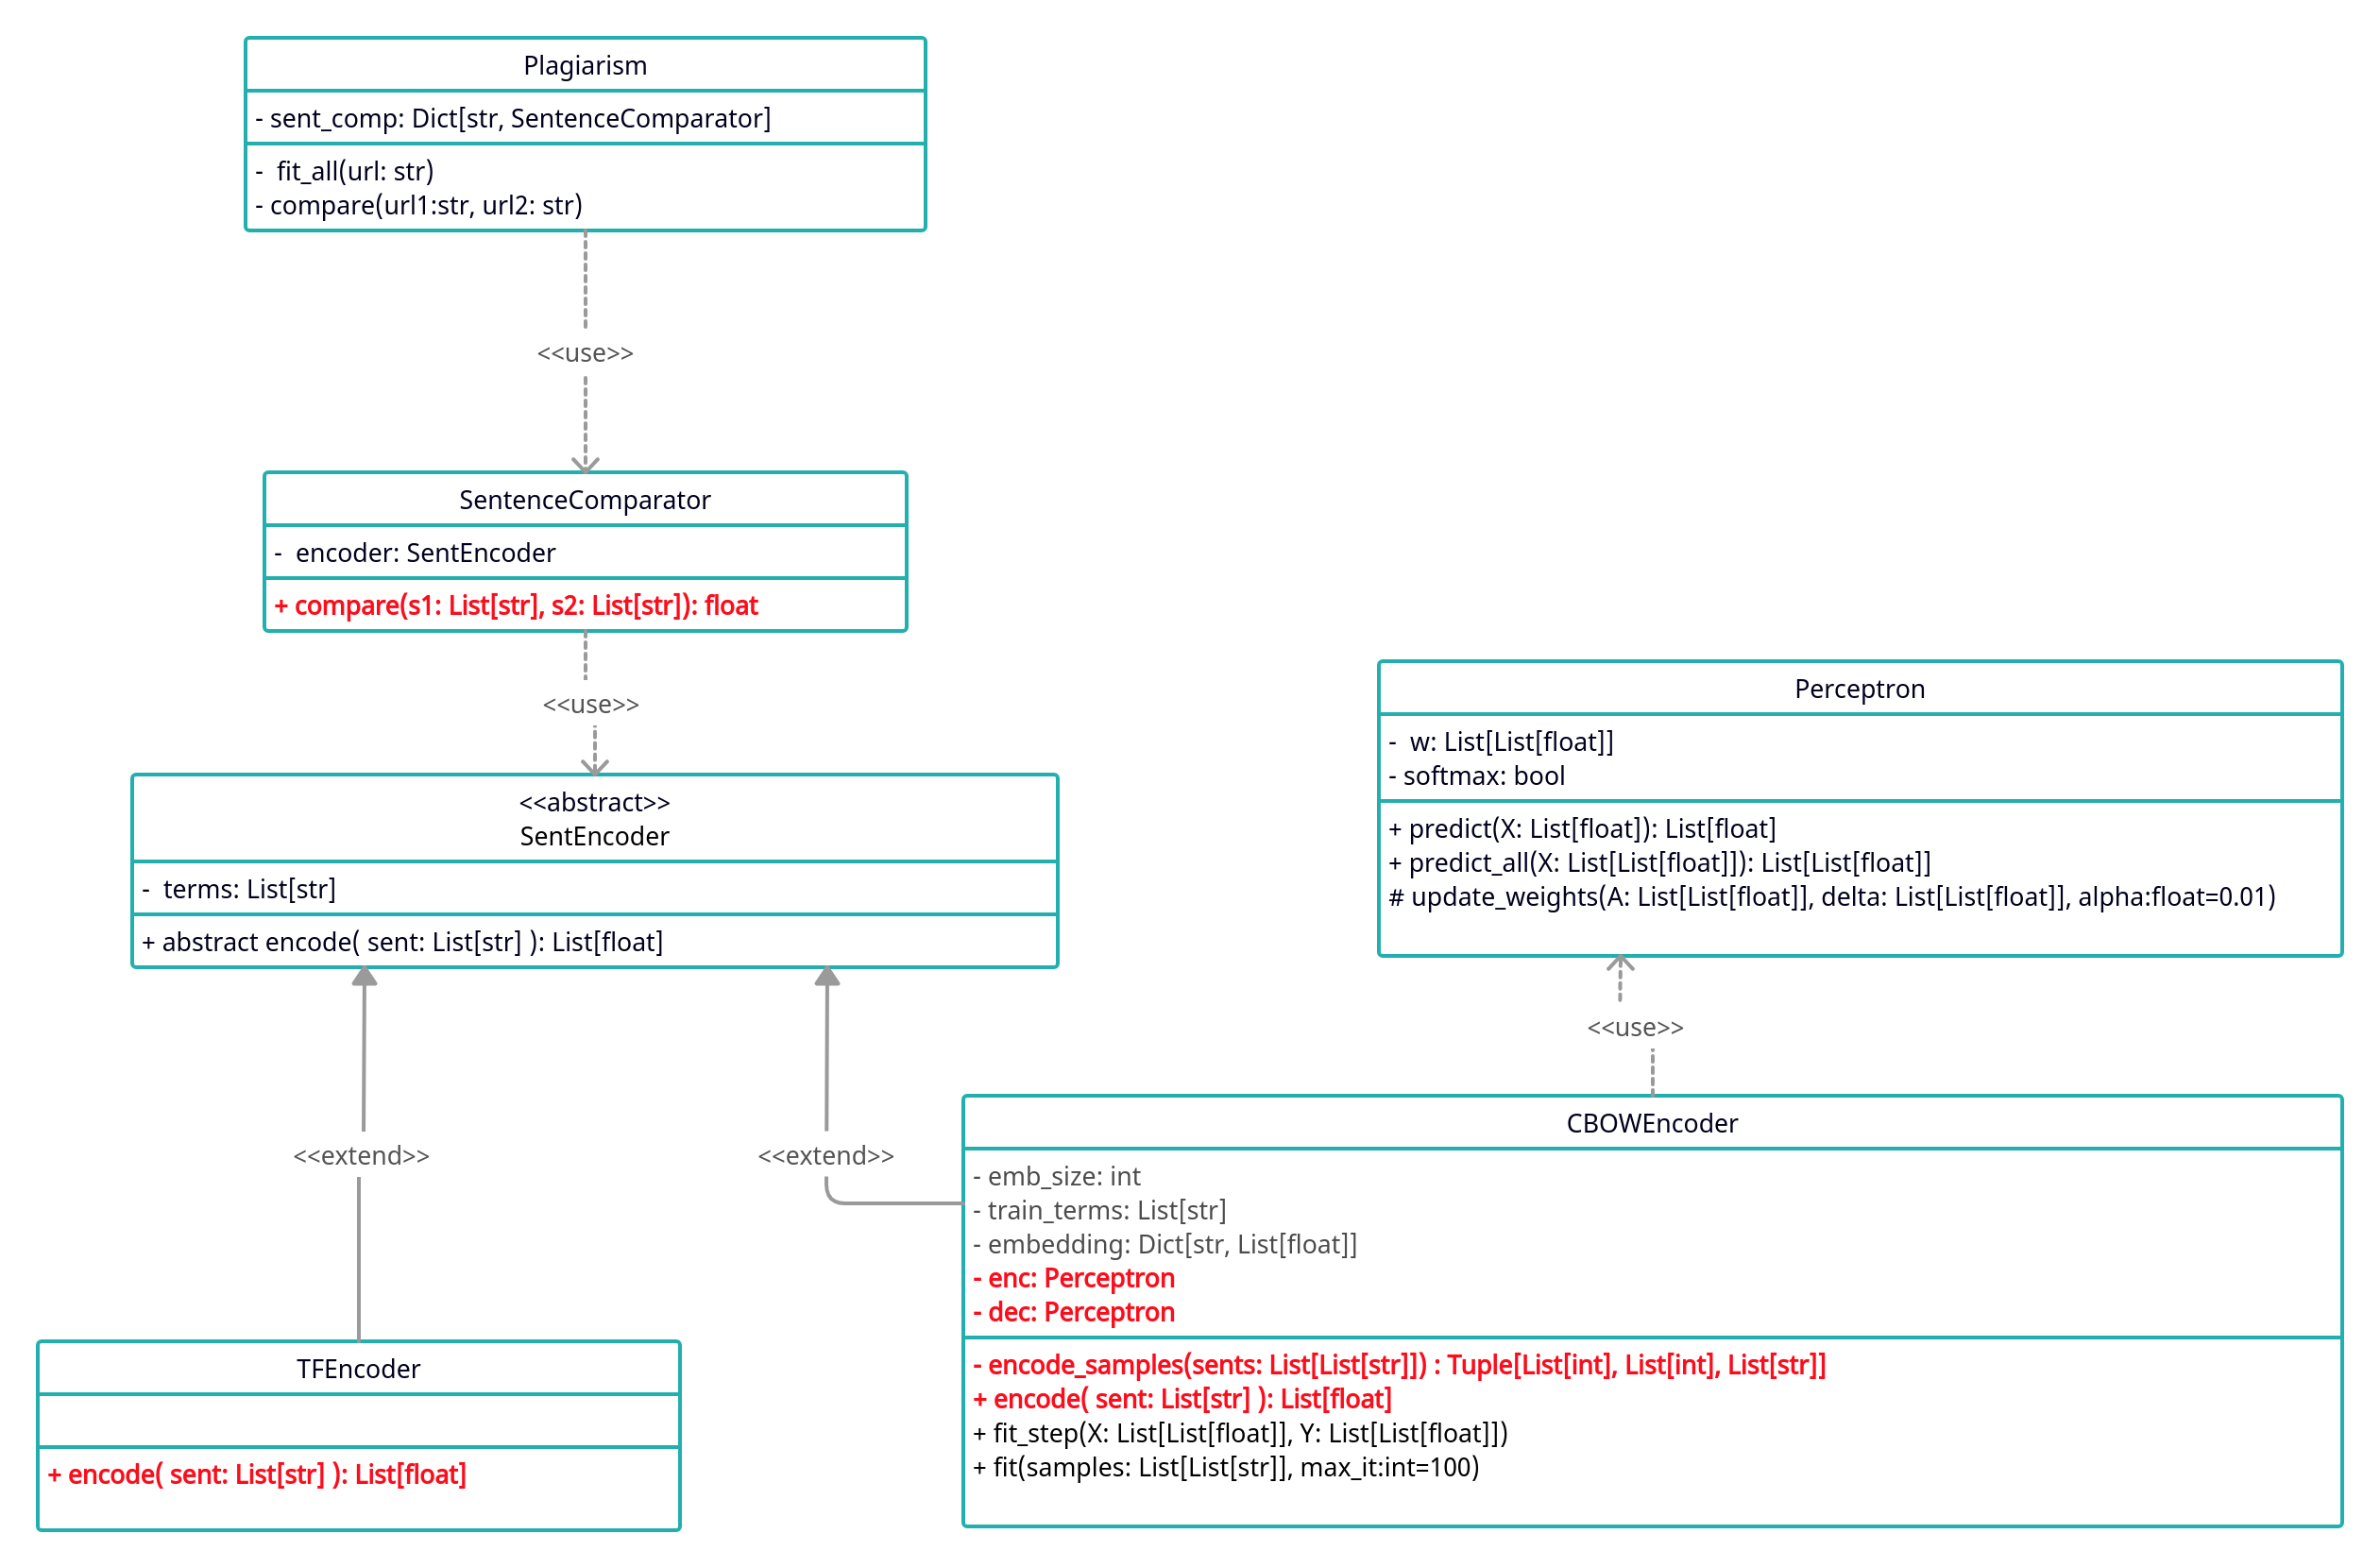
\includegraphics[width=0.8\textwidth]{./Lab4.png}
	\caption{Class diagram of our plagiarism program}
	\label{fig:program}
\end{figure}

\subsection{SentEncoder class}

It is an abstract class which stores the list of terms \textbf{"terms"} which will be used to encode sentences.
Also, it specifies an abstract method \textbf{"encode"} which encodes a tokenized sentence into a vector.


\subsection{TFEncoder class}

It inherits from the class \textbf{"SentEncoder"}. 
It also overrides its abstract method \textbf{\textit{\color{red}which you have to implement}}.
This method is specified as follows:
\begin{itemize}
	\item It takes as input a tokenized sentence: list of words.
	\item It calculates the frequency of each term in this sentence. The encoding follows the order of the parent list \textbf{"terms"}.
	\item If a sentence's word does not exist in the terms list, we ignore it.
\end{itemize}

\subsection{Perceptron class}

It implements a perceptron layer which has these properties:
\begin{itemize}
	\item It contains a number \textbf{"size"} of neurons (output).
	\item It has an input of \textbf{"nb\_feat"}.
	\item It defines two activation functions: softmax (\textbf{softmax=True}) or linear (\textbf{softmax=False})
	\item To predict its output, either we use \textbf{"predict"} for one sample, or \textbf{"predict\_all"} for many.
\end{itemize}

\subsection{CBOWEncoder class}

It inherits from the class \textbf{"SentEncoder"}. 
It also overrides its abstract method \textbf{\textit{\color{red}which you have to implement}}.
Also, you have to implement a preprocessing method called \textbf{encode\_samples}.

\subsubsection{encode\_samples}

This method has these properties:
\begin{itemize}
	\item It takes a list of tokenized sentences.
	\item It encodes each past word and next word as a sample of $X$ using onehot over \textbf{"train\_terms"}.
	\item It extracts current word into a list $L$ and encode it as onehot over \textbf{"terms"} into $Y$.
\end{itemize} 

\subsubsection{encode}

This method is specified as follows:
\begin{itemize}
	\item It takes as input a tokenized sentence: list of words.
	\item It searches for the embedding of each word in the attribute \textbf{"embedding"}, otherwise the word will be ignored.
	\item It calculates the centroid of the embeddings.
	\item If no word has an embedding, it returns a vector of zeroes having the same size as embeddings.
\end{itemize}


\subsubsection{CBOW model}

In addition, you have to complete the CBOW architecture which is composed of two perceptrons: an encoder and a decoder.
The encoder is specified as:
\begin{itemize}
	\item It takes as input the past word and the next word encoded using onehot over the \textbf{"train\_terms"} which gives a vector $X$.
	\item It encodes them into a vector of size \textbf{"emb\_size"} following this equation:
	\[E = W_e X + B_e\]
\end{itemize}
The decoder is specified as:
\begin{itemize}
	\item It takes as input the encoded vector $E$.
	\item It decodes it into probabilities over \textbf{"terms"} (we do not generate paddings) following this equation:
	\[\hat{Y} = Softmax(W_d E + B_d)\]
\end{itemize}


\subsection{SentenceComparator class}

This class stores a sentence encoder to encode a given sentence. 
It offers the method \textbf{"compare" \textit{\color{red}which you have to implement}}.
This is a brief description of this method:
\begin{itemize}
	\item It takes two tokenized sentences and encodes them into two vectors using the previous encoder.
	\item It calculates cosine similarity between the two vectors, say X and Y.
	\[Cosine(X, Y) = \frac{X \cdot Y}{||X||\ ||Y||}\] 
	\item If the nominator or the denominator is null, it returns 0.
\end{itemize}

\subsection{Plagiarism class}

This class trains many sentence comparators which are stored in a dictionary.
Then, given two text files, it compares their sentences one to one using the different comparators.

\section{Questions}

Answer these questions at the beginning of your code, as comments:
\begin{enumerate}
	\item Why the two sentences "cats chase mice" and "mice chase cats" are considered similar 
	using both encodings (TF and CBOW)?
	Propose a solution to fix this.
	
	\item Why "cats chase mice" and "I fish" are having some similarity using CBOW ?
	
	\item "mice consume fish" and "rodents eat sardines" are quit similar.
	But using CBOW, they are not that similar.
	Why?
	Propose a different model which reflects this similarity.
	
\end{enumerate}


\section{Students' Grading}

\begin{itemize}
	\item Duration: 1h25m (including download, reading, realization and upload time)
	\item Grade
	\begin{itemize}
		\item \textbf{TFEncoder.encode} (3pts) = vector size is terms size (0.5pts) + right encoding (2pts) + none terms words not considered (0.5pts).
		\item \textbf{CBOWEncoder.encode\_samples} (4pts) = X encoding (2pts) + Y encoding (1pt) + L generation (1pt).
		\item \textbf{CBOWEncoder.encode} (3pts) = centroid (1pt) + no embedding (1pt).
		\item \textbf{CBOWEncoder model} (2pts) = encoder (1pt) + decoder (1pt).
		\item \textbf{SentenceComparator.compare} (3pts) = cosine similarity (2pts) + special case (1pt).
		\item \textbf{questions grade} (3pts) = 1pt each.
		\item \textbf{In time grade} (2pts) = you have to return the homework at time. 
		After 5 minutes, each minute is -0.25.
		Then, you'll have a 0.
	\end{itemize}
\end{itemize}

\section{Useful functions}

There are some implemented functions, you may use:
\begin{itemize}
	\item onehot(lst: List[Any], e: Any) -> List[int] : onehot representation of an element based on a list.
	\item vec\_plus(X: List[float], Y: List[float]) -> List[float]: element-wise addition.
	\item vec\_divs(X: List[float], s: float) -> List[float]: division of a vector on a scalar.
\end{itemize}

\end{document}
